\documentclass[12pt,a4paper]{article}
\usepackage[utf8]{inputenc}
\usepackage{graphicx}
\graphicspath{{../Images/}}
\usepackage{amsmath}
\usepackage{amsfonts}
\usepackage{amssymb}
\usepackage{hyperref}
\usepackage[margin=1in]{geometry}
\usepackage{subfig}
\usepackage{float}
\usepackage{xcolor}
\usepackage{listings}
\definecolor{dkgreen}{rgb}{0,0.6,0}
\definecolor{gray}{rgb}{0.5,0.5,0.5}
\definecolor{mauve}{rgb}{0.58,0,0.82}

\lstset{frame=tb,
  backgroundcolor=\color[rgb]{0.9,0.9,0.9},
  language=Python,
  aboveskip=3mm,
  belowskip=3mm,
  showstringspaces=false,
  columns=flexible,
  basicstyle={\small\ttfamily},
  numbers=none,
  numberstyle=\tiny\color{gray},
  keywordstyle=\color{blue},
  commentstyle=\color{dkgreen},
  stringstyle=\color{mauve},
  breaklines=true,
  breakatwhitespace=true,
  tabsize=3
}

\author{Thibaut Marmey}

\title{Notes de cours CADL - session-1\\
\normalsize \href{https://www.kadenze.com/courses/creative-applications-of-deep-learning-with-tensorflow-iv/sessions/introduction-to-tensorflow}{cours Kadenze - session-1}}

\begin{document}
	\maketitle

\begin{scriptsize} \begin{itemize}
\item Learn the basic idea behind machine learning: learning from data and discovering representations
\item Learn how to preprocess a dataset using its mean and standard deviation
\item Learn the basic components of a Tensorflow Graph
\end{itemize}\end{scriptsize}

\begin{normalsize}
\tableofcontents
\end{normalsize}

\section{Introduction}
\subsection{Généralités}
\begin{itemize}
\item Deep-learning in a type of Machine Learning
\item \textit{Deep} because it is composed of many layers of \textit{Neural Networks}
\item Other valuable branches of Machine Learning :
\begin{itemize}
\item Rinforcement Learning
\item Dictionary Learning
\item Probabilistic Graphical Models and Bayesian Methods (Bishop)
\item Genetic and Evolutionary Algorithms
\end{itemize}
\item The differents ways an object can appear in an image is called \textit{invariance}
\item The dataset teaches the algorithm how to see the world, but only the world of this dataset
\item Existing data :
\begin{itemize}
\item MNIST
\item CalTech
\item CelebNet
\item \href{http://www.image-net.org/}{ImageNet}
\item LFW
\item CIFAR10, CIFRA100, \href{http://mscoco.org/home/}{MS Coco}...
\end{itemize}
\end{itemize}


\subsection{Preprocessing Data}
\begin{itemize}
\item Collect the images into a batch configuration. With this configuration, it's easier to make some computation over all the data.\\
This means, the data is in a single \textit{numpy} variable : \textit{data = np.array(imgs)}
\item Compute the Mean and Deviation of Images (of the batch channel)
\begin{itemize}
\item \begin{lstlisting}
mean_img = np.mean(data, axis=0) #mean of each col
plt.imshow(mean_img.astype(np.uint8))
\end{lstlisting}
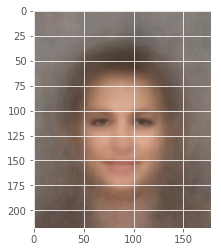
\includegraphics[scale=0.5]{dataMean}\\
This describes what most the dataset looks like.
\item \begin{lstlisting}
std_img = np.std(data, axis=0)
plt.imshow(std_img.astype(np.uint8))
\end{lstlisting}
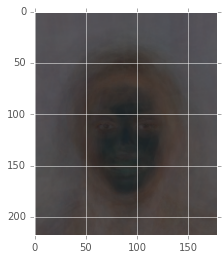
\includegraphics[scale=0.5]{dataStd}\\
This describes where the changes are the most likely to appear in the dataset of images.
\item \begin{lstlisting}
plt.imshow(np.mean(std_img, axis=2).astype(np.uint8))
\end{lstlisting}
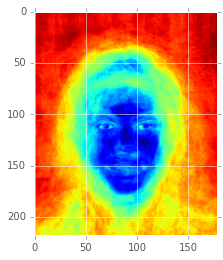
\includegraphics[scale=0.5]{dataStdMean}\\
This describes how every color channel will vary as a heatmap.
\begin{itemize}
\item Red part : not the best representation of the image
\item Blue part : the less likely that our mean image is far off from any other possible image
\end{itemize}
\end{itemize}
\end{itemize}

\subsection{Dataset preprocessing}
\begin{itemize}
\item We are trying to build a model that understands invariances (different of vision of an object, localization in the image, etc...)
\item If we use DL to learn something complex in the data, it starts by modeling both the mean and standard deviation or our dataset.
\item Speed up by "preprocessing" the dataset by removing the mean and standard deviation : it's called \textit{normalization}.\\
Subsctracting the mean and dividing by the standard deviation.
\item Look at the dataset with another way : array into a 1 dimensional array.
\begin{lstlisting}
flattened = data.ravel()
\end{lstlisting}
\item Visualize the \textbf{"distribution"}, or range and frequence of possible values. This tell us if \textbf{the data is predictable or not}.\\
\textit{plt.hist(data.ravel(), n} takes the min and max values of the \textit{data} array, and divide this interval in \textit{n} subintervals.
\begin{lstlisting}
plt.hist(flattened.ravel(), 255) #values are grouping in 255 bins
\end{lstlisting}
It tells us if something seems to happen more than anything else. If it does, the neural network will take advantage of that.
\item Normalization :
\begin{lstlisting}
plt.hist(((data[0] - mean_img) / std_img).ravel(), bins)
\end{lstlisting}
The data has been squished into a peak. Change the scale of the hist.\\
The data is concentrated between two values. The effect of normalizing : most of the data will be around 0, where some deviations of it will follow between the two values.\\
\begin{minipage}{\linewidth}
  \begin{figure}[H]
  \centering
    \subfloat[]{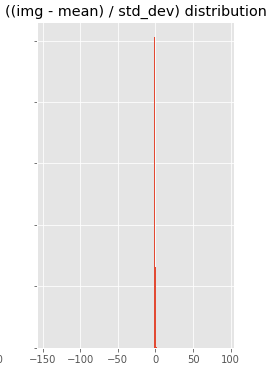
\includegraphics[scale=0.4]{normalizationPeak}}\hspace{1cm}
    \subfloat[]{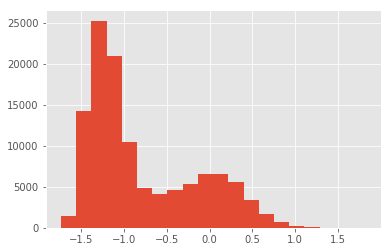
\includegraphics[scale=0.4]{normalizationPeakScaled}}
  \end{figure}
\end{minipage}
\item If the normalization doesn't look like this :
\begin{itemize}
\item get more data to calculate our mean/std deviation
\item try another method of normalization
\item not bother with normalization at all
\end{itemize}
\item Other options of normalization :
\begin{itemize}
\item local contrast normalization for images
\item PCA based normalization
\end{itemize}
\end{itemize}

\section{Tensorflow Basics}
\subsection{Basics}
\begin{itemize}
\item Working with Google's Library for Numerical Computation, TensorFlow
\item Different approach for doing the things above.
\item Instead of computing things immediately, we first define things that we want to compute later using what's called a \textit{Graph}.
\item Import the tensorflow library
\begin{lstlisting}
import tensorflow as tf
\end{lstlisting}
\item Range of numbers 
\begin{itemize}
\item with \textit{numpy} :
\begin{lstlisting}
np.linspace(-n, n, nbSubIntervals) #return list of 100 float64
\end{lstlisting}
\item with \textit{Tensorflow} :
\begin{lstlisting}
x = tf.linspace(-n,n,nbSubIntervals)
#return Tensor("LinSpace:0", shape=(100,), dtype=float32)
\end{lstlisting}
\begin{itemize}
\item \textit{LinSpace} : name
\item \textit{shape} : dimension and the number of values
\item \textit{dtype} : type of the values
\end{itemize}
\end{itemize}
\item \textit{tf.Tensor} and \textit{numpy.array} return different type of values.\\
No values printed because it actually hasn't computed its values yet. It just refers to the output of a \textit{tf.Operation}, already added to TF's default computational \textbf{graph}.\\
The result is the returned \textbf{Tensor object}.
\item Inspect "default" graph where all the operation have been added :
\begin{lstlisting}
tf.get_default_graph()
\end{lstlisting}
\begin{itemize}
\item Get the list of all added operation.
\begin{lstlisting}
[op.name for op in g.get_operations]
\end{lstlisting}
\end{itemize}
\item The result of a \textit{tf.Operation} is a \textit{tf.Tensor}
\item Create a \textit{tf.Session} to actually compute anything. It is responsible for evaluating the \textit{tf.Graph}.
\begin{lstlisting}
sess = tf.Session()	#create session
#compute anything created in the tensorflow graph
commputed_x = sees.run()
sess.close()	#close session
\end{lstlisting}
\item In iPython's interactive console, create an \textit{tf.InteractiveSession}
\begin{lstlisting}
sess = tf.InteractiveSession()
#The session is open for the rest of the lecture in Jupyter
x.eval()
\end{lstlisting}
\item Access to the shape : \textit{x.get\_shape()}
\item Create Gaussian curve (also refered by \textit{bell curve} or \textit{normal curve)}. It should resemble a normalized histogram. It needs two variables \textit{the mean value} (the curve is centred on it) and \textit{the standard deviation}.
\begin{lstlisting}
mean = 0.0
sigma = 1.0
z = (tf.exp(tf.negative(tf.pow(x - mean, 2.0) / (2.0 * tf.pow(sigma, 2.0)))) * (1.0 / (sigma * tf.sqrt(2.0 * 3.1415))))
\end{lstlisting}
Nothing has been computed. Just added operations to TF's graph. If we want the value or output, we have to ask the part of the graph we are interested. 
\item Interactive session is already created, call the \textit{eval()} function on the name of the  interested Tensor.
\end{itemize}

\subsection{Convolution}
\begin{itemize}
\item Creating a 2-D Gaussian Kernel. Can be done by multiplying a vector by its transpose.\\
\textit{tf.reshape(tensor, list)}
\begin{lstlisting}
# Let's store the number of values in our Gaussian curve.
ksize = z.get_shape().as_list()[0]
# Let's multiply the two to get a 2d Gaussian
z_2d = tf.matmul(tf.reshape(z, [ksize, 1]), tf.reshape(z, [1, ksize]))
# Execute the graph
plt.imshow(z_2d.eval())
\end{lstlisting}
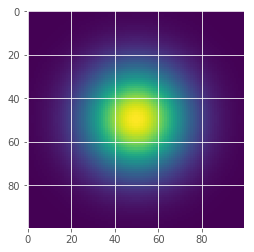
\includegraphics[scale=0.5]{gaussianKernel}
\item Common operation in DL : \textbf{convolution}\\
A way of filtering information. \href{http://setosa.io/ev/image-kernels/}{Here a link to visualize gaussian filters.}
\item Import a RGB image and convert it in a grayscale image with \textit{scikit-image} library.
\begin{lstlisting}
from skimage import color
from skimage import io
img = color.rgb2gray(io.imread('file')).astype(np.float32)
# Think to convert in np.float32 !
plt.imshow(img, cmap='gray')
\end{lstlisting}
The shape of \textit{img} is 2D. For image convultion with TF we need the batch dimension (N*H*W*C). With one grayscale image the shape is 1*H*W*1 (1 image, 1 channel).\\
Let's use the TF reshape function :
\begin{lstlisting}
img_4d = tf.reshape(img, [1, img.shape[0], img.shape[1], 1])
#Tensor("Reshape_50:0", shape=(1, 1920, 1920, 1), dtype=float32)
# float32 ok !
\end{lstlisting}
\item Reshape Gaussian Kernel to 4d (batch dimension) but the kernel dimension is different : \\
\textit{Kernel Height * K\_W * Number of Input Channels * Num of Output Channels}
\begin{lstlisting}
z_4d = tf.reshape(z_2d, [ksize, ksize, 1, 1])
\end{lstlisting}
\item Convolve image with Gaussian Kernel
\begin{lstlisting}
convolfed = tf.nn.conv2D(img_4D, strides=[1,1,1,1], pading='SAME')
\end{lstlisting}
\begin{itemize}
\item \textit{strides} : how to move our kernel across the image. Basically, two sets of parameters :
\begin{itemize}
\item \textbf{}[1, 1, 1, 1], which means, we are going to convolve every single image, every pixel, and every color channel by whatever the kernel is.
\item \textbf{}[1, 2, 2, 1], which means, we are going to convolve every single image, but every other pixel, in every single color channel.
\end{itemize}
\item \textit{padding} : what to do at the borders :
\begin{itemize}
\item \textit{'SAME'}, same dimensions as the original image (same dimensions going in and going out)
\item \textit{'VALID'}, the dimensions going out will change
\end{itemize}
\end{itemize}
\item Modulating the Gaussian with a Sine wave to create Gabor Kernel\\
Convolution kernel called a Gabor : like the Gaussian Kernel but using a sine wave to modulate.
\item Create an interval from -n to +n standard deviations with nb subintervals and the sin wave.
\begin{lstlisting}
xs = tf.linspace(-n, +n, nb)
ys = tf.sin(xs)
ys = tf.reshape(ys, [ksize, 1])
ones = tf.ones((1, ksize))
wave = tf.matmul(ys, ones)
\end{lstlisting}
\item Create the Gabor Kernel with the sin wave created before
\begin{lstlisting}
gabor = tf.multiply(wave, z_2d) #z_2d 2d-Gaussian
# tf.multiply() does element-wise multiplication
# tf.matmul() does matrix multiplication
\end{lstlisting}
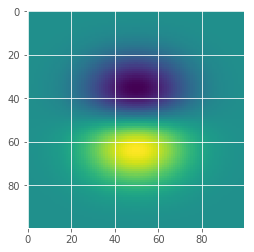
\includegraphics[scale=0.5]{gaborKernel}
\item Placeholders \textit{tf.placeholder(type, shape= , name=)} : specifying in our graph which elements we wanted to be specified later. Not sure what these are yet but we know they will fit in the graph (generally the input and output of the network).
\item Rewrite convolution using placeholder for the image and the kernel and setting image dimensions to \textit{None*None} (special for placeholders).
\begin{lstlisting}
# This is a placeholder which will become part of the tensorflow graph, but which we have to later explicitly define whenever we run/evaluate the graph.
img = tf.placeholder(tf.float32, shape=[None, None], name='img')
\end{lstlisting}
\item Reshape 2d image to a 3d tensor and again to batch dimension using \\
\textit{tf.expand\_dims(img, axis)}.\\
At the axis the channel dimension of 1 is added.
\begin{lstlisting}
# before dim : H * W
img_3d = tf.expand_dims(img, 2)
# img_3d.get_shape() = H * W * 1
img_4d = tf.expand_dims(img_4d, 0)
# img_4d.get_shape() = 1 * H * W * 1
\end{lstlisting}
\item Create another set of placeholders for Gabor's parameters
\begin{lstlisting}
mean = tf.placeholder(tf.float32, name='mean')
sigma = tf.placeholder(tf.float32, name='sigma')
ksize = tf.placeholder(tf.float32, name='ksize')
\end{lstlisting}
\item Redo the commands to build 2d gaussian kernel, sin wave, and finally \textit{gabor\_4d} :
\begin{lstlisting}
gabord_4d = tf.reshape(gabor, [ksize, ksize, 1,1])
\end{lstlisting}
\item At the end, do the convolution :
\begin{lstlisting}
convolved = tf.nn.conv2d(img_4d, gabor_4d, strides=[1, 1, 1, 1], padding='SAME', name='convolved')
convolved_img = convolved[0, :, :, 0]
\end{lstlisting}
\item At this point, not able to compute the convolution \textit{convolved\_img.eval()} because we have to specify all the placeholders required for the computation.\\
Get the error : "feed value for placeholder tensor".
\item Feed a value :
\begin{lstlisting}
res = convolved_img.eval(feed_dict={
		img: data.camera(), 
		mean:0.0, sigma:1.0, 
		ksize:100
		})
\end{lstlisting}
\end{itemize}

\section{Homework}
\subsection{Create a small dataset}
\begin{itemize}
\item Use extension of chrome web store : \href{https://chrome.google.com/webstore/detail/download-all-images/ifipmflagepipjokmbdecpmjbibjnakm?hl=en}{link}
\item Dataset download : images with cats
\item Load the dataset and create a 4d array (batch dimension):
\begin{lstlisting}
# load image from directory
filenames = [os.path.join('dirname', fname) for fname in os.listdir(dirname)]
# In filenames, we have the link of each pictures
# Read every filename as an RGB image
imgs = [plt.imread(fname)[:,:,:3] for fname in filenames]
# Crop the picture to square and the same size (size, size)
------
# Create the 4-D array like (number of images * H * W * color)
# And convert in np.float32
imgs = np.array(imgs).astype(np.float32)
\end{lstlisting}

\end{itemize}

\end{document}